
\section{Organic Semiconductors}
\label{sec:organic_semiconductors}

\begin{figure}[h]
    \centering
    \begin{minipage}{0.48\textwidth}
        \centering
        \resizebox{0.95\linewidth}{!}{\setchemfig{cram width=4pt, atom sep=1.7em}
\chemfig{
  H_{17}C_8-[:17]*6(-=*5(-{\color{red}S}-*5(-*6(-=-(-C_8H_{17})=-=)--{\color{red}S}-=)--)-=-=)
}
}\par
        \vspace{0.5em}
        C8-BTBT
    \end{minipage}\hfill
    \begin{minipage}{0.48\textwidth}
        \centering
        \resizebox{0.95\linewidth}{!}{\setchemfig{cram width=4pt, atom sep=1.7em}
\par\vspace{1em}\noindent
\chemfig{
  H_{25}C_{12}-[:17]*6(-=*5(-{\color{red}S}-*5(-*6(-=-(-C_{12}H_{25})=-=)--{\color{red}S}-=)--)-=-=)
}}\par
        \vspace{0.5em}
        C12-BTBT
    \end{minipage}

    \vspace{1em}

    \begin{minipage}{0.4\textwidth}
        \centering
        \resizebox{0.95\linewidth}{!}{\setchemfig{cram width=4pt, atom sep=1.7em}
\par\vspace{1em}\noindent
\chemfig{
  [:0]*6(=-*6(=-*5(-*5(-{\color{red}S}-*6(-=*6(-=-=-=)-=-=)=--)=-{\color{red}S}--)=-=-)--=-)
}
}\par
        \vspace{0.5em}
        DNTT
    \end{minipage}\hspace{18mm}
    \begin{minipage}{0.4\textwidth}
        \centering
        \resizebox{0.95\linewidth}{!}{\setchemfig{cram width=4pt, atom sep=1.7em}
\chemfig{
  [:-13]*6(-=*5(-{\color{red}S}-*5(-*6(-=-(-*6(=-=-=-))=-=)--{\color{red}S}-=)--)-=-=)
}
}\par
        \vspace{0.5em}
        Ph-BTBT
    \end{minipage}
    \caption[Chemical structures of common organic semiconductors]{Chemical
    structures of common high-mobility small-molecule organic semiconductors:
    C8-BTBT, C12-BTBT, DNTT, and Ph-BTBT.}
    \label{fig:organic_semiconductor_examples}
\end{figure}

Organic semiconductors are carbon-based molecular or polymeric materials in
which electronic transport is governed by conjugated $\pi$-electron systems.
Unlike inorganic semiconductors, where atoms are connected by strong covalent
bonds throughout a crystal lattice, organic semiconductors are usually held
together by weaker intermolecular interactions. The resulting electronic
coupling between molecules is comparatively small, so charge transport is highly
sensitive to molecular packing, energetic disorder, defects, interfaces, and trap
states~\cite{Bruetting2005,Coropceanu2007ChargeTransport}. Representative high-mobility small-molecule organic semiconductors, including
BTBT derivatives and DNTT, are shown in
Figure~\ref{fig:organic_semiconductor_examples}~\cite{Wang2017LowVoltageC8BTBT,Sirringhaus2005DevicePhysics}.

For this thesis, the relevant physical picture is that the gate voltage and the
contacts determine how many carriers are injected or accumulated, while the
molecular solid determines how efficiently those carriers move. The following
subsections summarize the molecular electronic structure, disorder and trap
states, carrier distribution in field-effect geometries, and temperature-dependent
transport mechanisms.

\subsection{Molecular Structure and Electronic States}
\label{subsec:molecular_structure_electronic_states}

The frontier molecular orbitals dominate the electronic properties of organic
semiconductors. The \textit{highest occupied molecular orbital} (HOMO) is analogous to the
valence band maximum of an inorganic semiconductor, while the \textit{lowest unoccupied molecular
orbital} (LUMO) is analogous to the conduction band minimum. Their energetic separation is
commonly called the transport gap,
\begin{equation}
    E_\mathrm{g} = E_\mathrm{LUMO} - E_\mathrm{HOMO} .
\end{equation}
For $p$-type materials, hole transport is associated mainly with HOMO-derived
states; for $n$-type materials, electron transport occurs through LUMO-derived
states~\cite{Bruetting2005,Coropceanu2007ChargeTransport}.

\begin{figure}[h]
    \centering
    \begin{minipage}{0.45\textwidth}
        \centering
        \resizebox{\textwidth}{!}{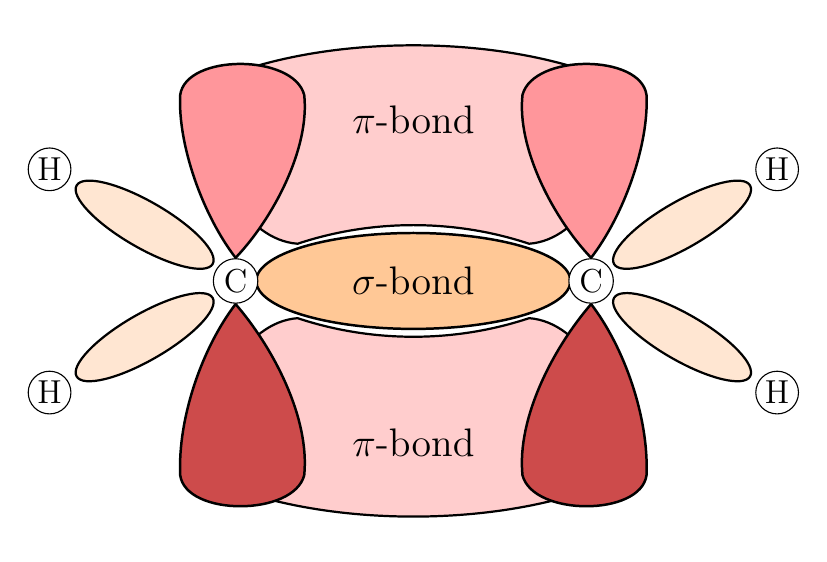
\begin{tikzpicture}[
    scale=1.05,
    every node/.style={font=\sffamily},
    line join=round,
    line cap=round
]

% Colors
\definecolor{pibond}{RGB}{255,205,205}
\definecolor{porbtop}{RGB}{255,150,155}
\definecolor{porbbot}{RGB}{205,75,75}
\definecolor{sigmabond}{RGB}{255,200,150}
\definecolor{hbond}{RGB}{255,230,210}


% ----------------------------------------------------
% Large pi bond regions, drawn first in background
% ----------------------------------------------------
\path[fill=pibond, draw=black, line width=0.8pt]
(-2.75,2.25)
.. controls (-1.35,3.05) and (1.35,3.05) .. (2.75,2.25)
.. controls (2.45,1.35) and (2.05,0.50) .. (1.40,0.45)
.. controls (0.50,0.75) and (-0.50,0.75) .. (-1.40,0.45)
.. controls (-2.05,0.50) and (-2.45,1.35) .. (-2.75,2.25)
-- cycle;

\path[fill=pibond, draw=black, line width=0.8pt]
(-2.75,-2.25)
.. controls (-1.35,-3.05) and (1.35,-3.05) .. (2.75,-2.25)
.. controls (2.45,-1.35) and (2.05,-0.50) .. (1.40,-0.45)
.. controls (0.50,-0.75) and (-0.50,-0.75) .. (-1.40,-0.45)
.. controls (-2.05,-0.50) and (-2.45,-1.35) .. (-2.75,-2.25)
-- cycle;

% ----------------------------------------------------
% Hydrogen sigma-like C--H bond clouds
% ----------------------------------------------------
\newcommand{\chcloud}[3]{%
\begin{scope}[shift={(#1,#2)}, rotate=#3]
\path[fill=hbond, draw=black, line width=0.8pt]
(0,0) ellipse[x radius=0.95, y radius=0.28];
\end{scope}
}

\chcloud{-3.25}{0.68}{150}
\chcloud{-3.25}{-0.68}{-150}
\chcloud{3.25}{0.68}{30}
\chcloud{3.25}{-0.68}{-30}

% ----------------------------------------------------
% 2pz orbitals
% ----------------------------------------------------
% left upper
\path[fill=porbtop, draw=black, line width=0.9pt]
(-2.15,0.28)
.. controls (-2.55,0.80) and (-2.85,1.65) .. (-2.82,2.25)
.. controls (-2.75,2.75) and (-1.45,2.75) .. (-1.32,2.25)
.. controls (-1.25,1.60) and (-1.70,0.75) .. (-2.15,0.28)
-- cycle;

% right upper
\path[fill=porbtop, draw=black, line width=0.9pt]
(2.15,0.28)
.. controls (2.55,0.80) and (2.85,1.65) .. (2.82,2.25)
.. controls (2.75,2.75) and (1.45,2.75) .. (1.32,2.25)
.. controls (1.25,1.60) and (1.70,0.75) .. (2.15,0.28)
-- cycle;

% left lower
\path[fill=porbbot, draw=black, line width=0.9pt]
(-2.15,-0.28)
.. controls (-2.55,-0.80) and (-2.85,-1.65) .. (-2.82,-2.35)
.. controls (-2.75,-2.85) and (-1.45,-2.85) .. (-1.32,-2.35)
.. controls (-1.25,-1.65) and (-1.70,-0.80) .. (-2.15,-0.28)
-- cycle;

% right lower
\path[fill=porbbot, draw=black, line width=0.9pt]
(2.15,-0.28)
.. controls (2.55,-0.80) and (2.85,-1.65) .. (2.82,-2.35)
.. controls (2.75,-2.85) and (1.45,-2.85) .. (1.32,-2.35)
.. controls (1.25,-1.65) and (1.70,-0.80) .. (2.15,-0.28)
-- cycle;

% ----------------------------------------------------
% sigma bond
% ----------------------------------------------------
\path[fill=sigmabond, draw=black, line width=0.9pt]
(0,0) ellipse[x radius=1.90, y radius=0.58];

% ----------------------------------------------------
% Carbon and hydrogen atoms
% ----------------------------------------------------
\node[circle, draw=black, fill=white, inner sep=1.5pt, font=\large] at (-2.15,0) {C};
\node[circle, draw=black, fill=white, inner sep=1.5pt, font=\large] at ( 2.15,0) {C};

\node[circle, draw=black, fill=white, inner sep=1.2pt, font=\large] at (-4.40,1.35) {H};
\node[circle, draw=black, fill=white, inner sep=1.2pt, font=\large] at (-4.40,-1.35) {H};
\node[circle, draw=black, fill=white, inner sep=1.2pt, font=\large] at ( 4.40,1.35) {H};
\node[circle, draw=black, fill=white, inner sep=1.2pt, font=\large] at ( 4.40,-1.35) {H};

% ----------------------------------------------------
% Labels
% ----------------------------------------------------
\node[font=\Large] at (0,1.95) {$\pi$-bond};
\node[font=\Large] at (0,0) {$\sigma$-bond};
\node[font=\Large] at (0,-1.95) {$\pi$-bond};



\end{tikzpicture}}
    \end{minipage}
    \hfill
    \begin{minipage}{0.51\textwidth}
        \centering
        \resizebox{\textwidth}{!}{\begin{tikzpicture}[
    scale=1.05,
    every node/.style={font=\sffamily},
    level/.style={line width=1pt},
    spin/.style={-{Latex[length=2mm]}, line width=0.9pt},
    excite/.style={-{Latex[length=2.5mm]}, dashed, line width=1pt, gray},
    brace/.style={decorate, decoration={brace, amplitude=5pt}},
]

% Required:
% \usepackage{tikz}
% \usetikzlibrary{arrows.meta,decorations.pathreplacing}

% Coordinates
\def\xL{1.2}
\def\xR{3.55}

\def\ysigma{0.0}
\def\ypi{1.05}
\def\ypistar{2.25}
\def\ysigstar{3.25}

% Energy axis
\draw[-{Latex[length=3mm]}, line width=1pt]
(0.35,-0.35) -- (0.35,3.65);

\node[rotate=90] at (0.0,1.6) {Energy};

% Energy levels
\draw[level] (\xL,\ysigstar) -- (\xR,\ysigstar);
\draw[level] (\xL,\ypistar)  -- (\xR,\ypistar);
\draw[level] (\xL,\ypi)      -- (\xR,\ypi);
\draw[level] (\xL,\ysigma)   -- (\xR,\ysigma);

% Orbital labels
\node[right] at (3.65,\ysigstar) {$\sigma^{\ast}$-orbital};
\node[right] at (3.65,\ypistar)  {$\pi^{\ast}$-orbital};
\node[right] at (3.65,\ypi)      {$\pi$-orbital};
\node[right] at (3.65,\ysigma)   {$\sigma$-orbital};

% Bonding and antibonding braces
\draw[brace] (5.5,\ysigstar+0.23) -- (5.5,\ypistar-0.23);
\node[right] at (5.75,2.75) {antibonding orbitals};

\draw[brace] (5.5,\ypi+0.23) -- (5.5,\ysigma-0.23);
\node[right] at (5.75,0.53) {bonding orbitals};

% Electron pairs in bonding orbitals
% sigma orbital
\draw[spin] (2.25,\ysigma-0.32) -- (2.25,\ysigma+0.32);
\draw[spin] (2.5,\ysigma+0.32) -- (2.5,\ysigma-0.32);

% pi orbital
\draw[spin] (2.25,\ypi-0.32) -- (2.25,\ypi+0.32);
\draw[spin] (2.5,\ypi+0.32) -- (2.5,\ypi-0.32);

% Optical excitation arrow
\draw[excite] (3.25,\ypi+0.1) -- (3.25,\ypistar-0.1);
\node[gray, font=\bfseries] at (5.25,1.62) {optical excitation};

\end{tikzpicture}}
    \end{minipage}
    \caption[Sigma and pi bonding in ethene]{Sigma and pi bonding in ethene as
    the simplest conjugated pi-electron system. The left panel illustrates the
    spatial overlap of the $\sigma$ and $\pi$ bonds, while the right panel shows
    the corresponding bonding and antibonding orbital levels. The lowest optical
    excitation occurs from the bonding $\pi$ orbital to the antibonding
    $\pi^{\ast}$ orbital. Adapted from Ref.~\cite{Riederer2023Dissertation} and \cite{Neamen}.}
    \label{fig:osemi_electron}
\end{figure}

The origin of semiconducting behaviour is $\pi$-conjugation. In conjugated
molecules, neighbouring carbon atoms are typically $sp^2$ hybridized, leaving
$p_z$ orbitals that overlap to form delocalized $\pi$ orbitals. Within one
molecule this delocalization can be strong, but transport through a solid also
requires overlap between orbitals on neighbouring molecules. Because this
intermolecular overlap is weak, small changes in molecular packing, tilt angle,
thermal motion, or grain orientation can strongly change the electronic transfer
integral and therefore the mobility~\cite{Coropceanu2007ChargeTransport}.

The basic bonding picture is illustrated in Figure~\ref{fig:osemi_electron}.
Ethene is the simplest example of a conjugated $\pi$-electron system: the
$\sigma$ bond forms the molecular backbone, while the $p_z$ orbitals combine
into bonding $\pi$ and antibonding $\pi^*$ orbitals. In longer conjugated
molecules, many such orbitals split into a set of occupied and unoccupied
levels. The lowest optical excitation is then typically associated with a
transition from the bonding $\pi$-derived HOMO to the antibonding
$\pi^*$-derived LUMO~\cite{Bruetting2005}.



Organic semiconductors are often classified as small molecules or conjugated
polymers. Small molecules can form crystals or polycrystalline films with grains
and grain boundaries, whereas polymers usually contain both ordered and
disordered chain segments. In both classes, improved molecular order generally
increases orbital overlap and reduces energetic disorder, but real thin films
remain strongly influenced by processing conditions and interfaces
~\cite{Bruetting2005,Sirringhaus2005DevicePhysics}.

\subsection{Energetic Disorder and Trap States}
\label{subsec:energetic_disorder_traps}

A real organic semiconductor thin film is not an ideal periodic crystal.
Variations in molecular position, orientation, grain structure, impurities,
interface roughness, and dielectric dipoles create local shifts of the HOMO and
LUMO energies. Therefore, the transport states are not represented by sharp band
edges. A common approximation for disordered organic semiconductors is a
Gaussian density of states (DOS),
\begin{equation}
    g(E) = \frac{N_0}{\sqrt{2\pi}\sigma_\mathrm{DOS}}
    \exp\left[-\frac{(E-E_0)^2}{2\sigma_\mathrm{DOS}^2}\right],
    \label{eq:gaussian_dos}
\end{equation}
where $N_0$ is the total density of localized states, $E_0$ is the centre of
the distribution, and $\sigma_\mathrm{DOS}$ describes the energetic disorder.
Tail states and additional deep traps can be superimposed on this Gaussian
background. This Gaussian-disorder picture is widely used to describe hopping
transport in organic semiconductors~\cite{Bassler1993ChargeTransport,Bruetting2005,Darwish2020DriftDiffusionOFET}.

Trap states are localized states that temporarily immobilize charge carriers. For
a $p$-type semiconductor, hole traps reduce the density of mobile holes; for an
$n$-type semiconductor, electron traps play the corresponding role. The total
carrier density can therefore be separated into mobile and trapped parts,
\begin{equation}
    n_\mathrm{tot} = n_\mathrm{free} + n_\mathrm{trap} .
\end{equation}
Only the mobile part contributes directly to the conductivity,
\begin{equation}
    \sigma = q n_\mathrm{free}\mu ,
\end{equation}
where $q$ is the elementary charge and $\mu$ is the effective mobility
~\cite{Bruetting2005,Hirwa2015TrapStates}.

Shallow traps lie close to the transport level and can release carriers by
thermal excitation. Deep traps are farther from the transport level and can store
charge for longer times. Deep or slowly exchanging traps can cause threshold
voltage shifts, hysteresis, bias-stress effects, and memory during cooling and
heating cycles. Consequently, temperature-dependent measurements probe not only a
mobility change, but also a redistribution of carriers between mobile and trapped
states~\cite{Hirwa2015TrapStates,Bobbert2012OperationalStability}.

 \subsection{Charge Carrier Distribution}
\label{subsec:charge_carrier_distribution}

Because many organic semiconductors have relatively large transport gaps, their
intrinsic thermally generated carrier density is small. In field-effect devices,
the relevant carrier density is mainly set by contact injection and by the gate
electric field. For a $p$-type semiconductor, a negative gate voltage attracts
holes to the semiconductor--dielectric interface and forms an accumulation layer;
for an $n$-type semiconductor, a positive gate voltage accumulates electrons
~\cite{Sirringhaus2005DevicePhysics,Bruetting2005}.

In the gradual-channel approximation, the induced sheet charge density can be
written as
\begin{equation}
    Q = C_\mathrm{i}\left(V_\mathrm{G}-V_\mathrm{T}-V\right),
    \label{eq:gate_charge}
\end{equation}
where $C_\mathrm{i}$ is the gate-insulator capacitance per unit area,
$V_\mathrm{G}$ is the gate voltage, $V_\mathrm{T}$ is an effective threshold
voltage, and $V$ is the local channel potential. The corresponding two-dimensional
carrier density is
\begin{equation}
    n_\mathrm{2D} = \frac{|Q|}{q}
    = \frac{C_\mathrm{i}}{q}\left|V_\mathrm{G}-V_\mathrm{T}-V\right| .
    \label{eq:carrier_density_2d}
\end{equation}
These relations show that the carrier density is not fixed only by the externally
applied gate voltage; it also varies along the channel through the local
potential. This point is important for transistor measurements and for gated van
der Pauw geometries, where the measured conductance corresponds to a specific
probed region of the film~\cite{Sirringhaus2005DevicePhysics,Rolin2017GVDP}.

Microscopically, the carrier density follows from the Gaussian DOS and the
Fermi--Dirac occupation. For electron transport through LUMO-derived states,
\begin{equation}
    n = \int_{-\infty}^{\infty} g_\mathrm{LUMO}(E)
    f(E,E_\mathrm{F},T)\,\mathrm{d}E,
\end{equation}
whereas the hole density in HOMO-derived states is
\begin{equation}
    p = \int_{-\infty}^{\infty} g_\mathrm{HOMO}(E)
    \left[1-f(E,E_\mathrm{F},T)\right]\,\mathrm{d}E .
\end{equation}
Here $g_\mathrm{HOMO}$ and $g_\mathrm{LUMO}$ are often modeled by Gaussian
distributions of the form of Equation~\ref{eq:gaussian_dos}. Shifting the Fermi
level by the gate field therefore changes both the number of mobile carriers and
the occupation of localized tail and trap states
~\cite{Stodtmann2012OrganicSimulation,Darwish2020DriftDiffusionOFET}.

\subsection{Charge Carrier Transport Mechanisms}
\label{subsec:charge_carrier_transport_mechanisms}

Charge transport in organic semiconductors is not described by a single universal
mechanism. The dominant process depends on molecular order, temperature,
energetic disorder, carrier density, and contact quality. In highly ordered
single crystals or well-ordered films, carriers can show band-like transport, in
which the mobility decreases with increasing temperature because molecular
vibrations disturb intermolecular electronic coupling. A common empirical form is
\begin{equation}
    \mu(T) \propto T^{-n},
\end{equation}
where $n>0$~\cite{Sakanoue2010BandLikeMobility,Coropceanu2007ChargeTransport}.

In more disordered thin films, transport is often described as hopping between
localized states. A hop depends on the distance between sites, their energy
difference, the electric field, and the thermal energy available to overcome
local barriers. Thermally activated hopping often gives a mobility that increases
with temperature and can be approximated by an Arrhenius relation,
\begin{equation}
    \mu(T) = \mu_0
    \exp\left(-\frac{E_\mathrm{a}}{k_\mathrm{B}T}\right),
    \label{eq:arrhenius_mobility}
\end{equation}
where $\mu_0$ is a prefactor and $E_\mathrm{a}$ is an effective activation
energy. This activation energy can include contributions from energetic disorder,
trap release, grain-boundary barriers, and contact injection
~\cite{Bassler1993ChargeTransport,Bruetting2005}.

In a band-transport picture, the mobility is limited by scattering processes that
reduce the average momentum-relaxation time $\tau$. The Drude relation
$\mu=q\tau/m^*$ therefore shows that stronger scattering directly lowers the
mobility. Two important limiting mechanisms are phonon scattering and ionized
impurity scattering. Phonon scattering is caused by lattice vibrations or, in
organic crystals, thermally excited molecular motions that modulate the
intermolecular transfer integrals. As the temperature increases, these vibrations
become stronger and the phonon-limited mobility typically decreases. In many
crystalline semiconductors this trend is written approximately as
$\mu_\mathrm{ph}\propto T^{-3/2}$, although the exact exponent depends on the
material and dominant phonon mode. Ionized impurity scattering originates from
the Coulomb potential of charged dopants, trapped charges, or fixed interface
charges. It becomes stronger when the concentration of charged scattering centers
increases and is often approximated by
$\mu_\mathrm{ii}\propto T^{3/2}/N_\mathrm{i}$, where $N_\mathrm{i}$ is the
ionized impurity concentration. If several independent scattering processes are
present, their contributions can be combined using Matthiessen's rule,
\begin{equation}
    \frac{1}{\mu_\mathrm{tot}} = \frac{1}{\mu_\mathrm{ph}}
    + \frac{1}{\mu_\mathrm{ii}} + \cdots .
\end{equation}
This relation shows that the smallest partial mobility, corresponding to the
strongest scattering channel, dominates the measured mobility. In organic thin
films these simple power laws should be interpreted qualitatively, because
energetic disorder, trapping, grain boundaries, and hopping transport often
contribute at the same time~\cite{Neamen,Bruetting2005,Coropceanu2007ChargeTransport}.

\begin{figure}[h]
    \centering
    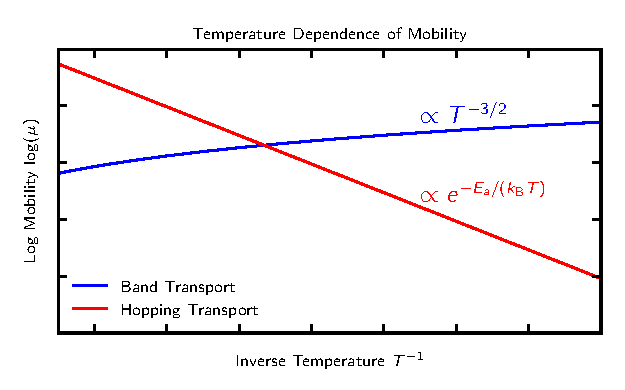
\includegraphics[scale=1]{figures/temp-dependence.eps}
    \caption[Temperature dependence of organic semiconductor transport]{Schematic
    temperature dependence of charge transport in organic semiconductors.
    Thermally activated hopping typically becomes more efficient at higher
    temperature, whereas band-like transport can decrease with increasing
    temperature because molecular vibrations disturb intermolecular coupling.}
    \label{fig:temp_dependence_transport}
\end{figure}
